A continuación se describen los ítems, cosméticos y tablas de recompensas que se han implementado en el MVP. E
stos elementos son fundamentales para enriquecer la experiencia de juego, ofreciendo a los jugadores diversas opciones para personalizar su personaje y 
obtener recompensas a medida que avanzan en el juego.

\subsubsection{Ítems}

Los ítems son elementos que los jugadores pueden recoger y utilizar durante el juego. Por el momento se 
ofrecen dos tipos:

\begin{itemize}
  \item \textbf{Objetos Consumibles (\textit{Consumable Items})}: son ítems que el jugador puede usar para obtener un efecto temporal,
como recuperar salud o aumentar la velocidad de movimiento. Son configurables en cuanto a tipo de consumible, efecto, duración y textura.

\begin{figure}[H]
\centering
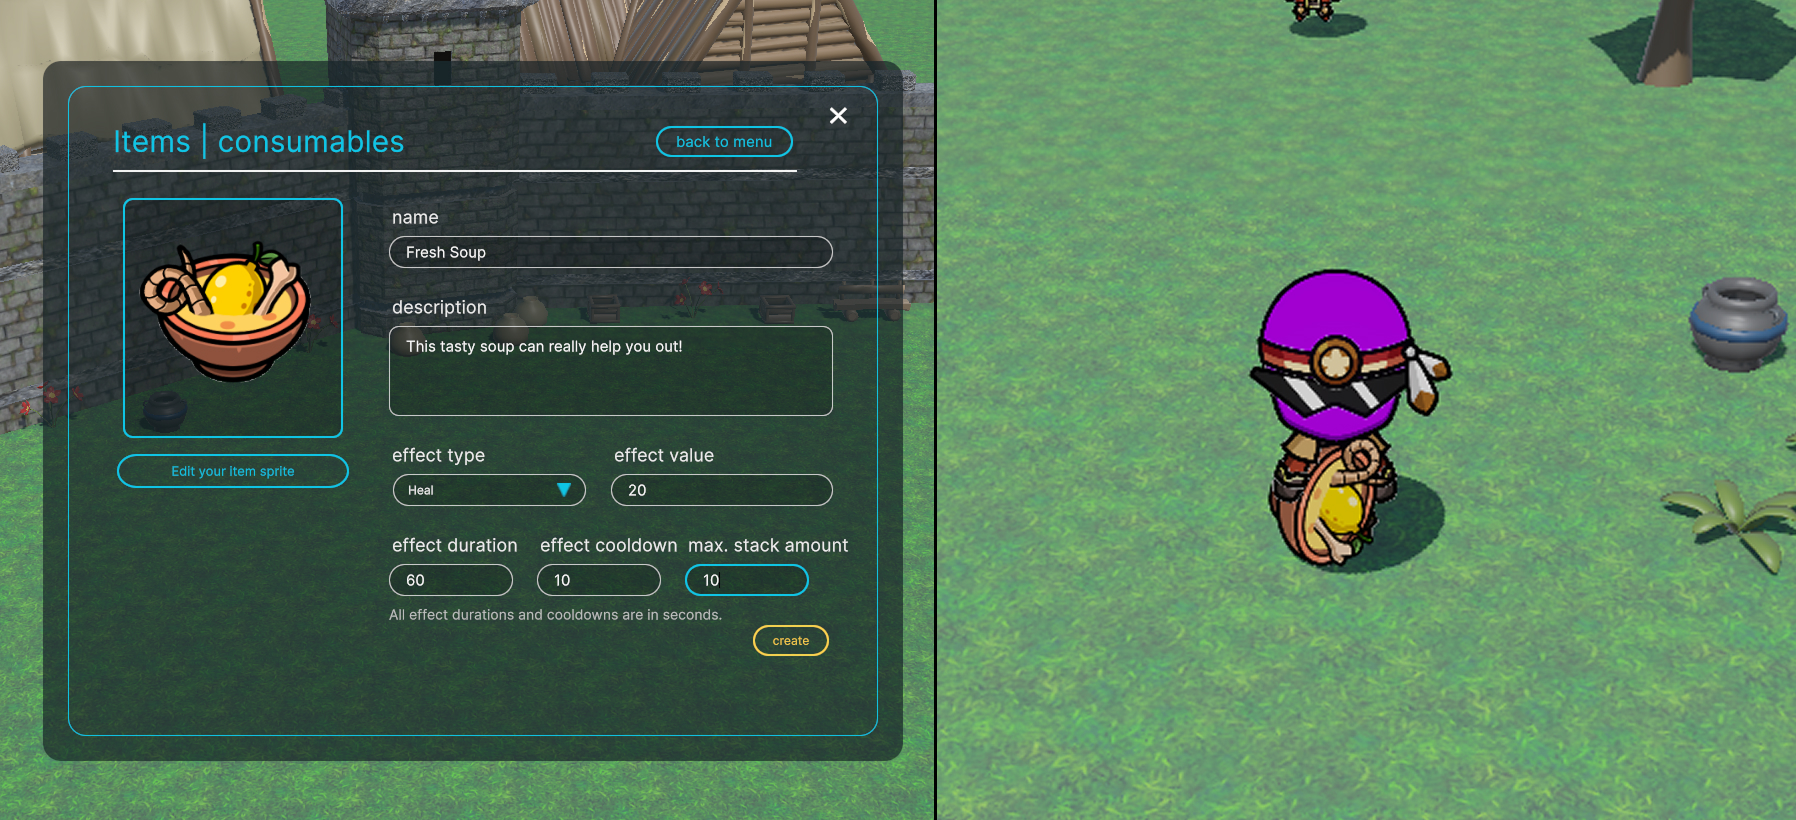
\includegraphics[width=0.90.9\textwidth]{img/08-implemented-solution/product/consumable-item.jpg}
\caption{Captura de un jugador interactuando con un objeto consumible y como se ve en el creador de mundos}
\end{figure}

\item \textbf{Armas (\textit{Weapon Items})}: ítems que el jugador puede equipar para atacar a enemigos u otros jugadores. Son configurables en cuanto a 
tipo de arma (\textit{melee} o a distancia), daño, alcance, velocidad de ataque y textura.
\end{itemize}

\begin{figure}[H]
\centering
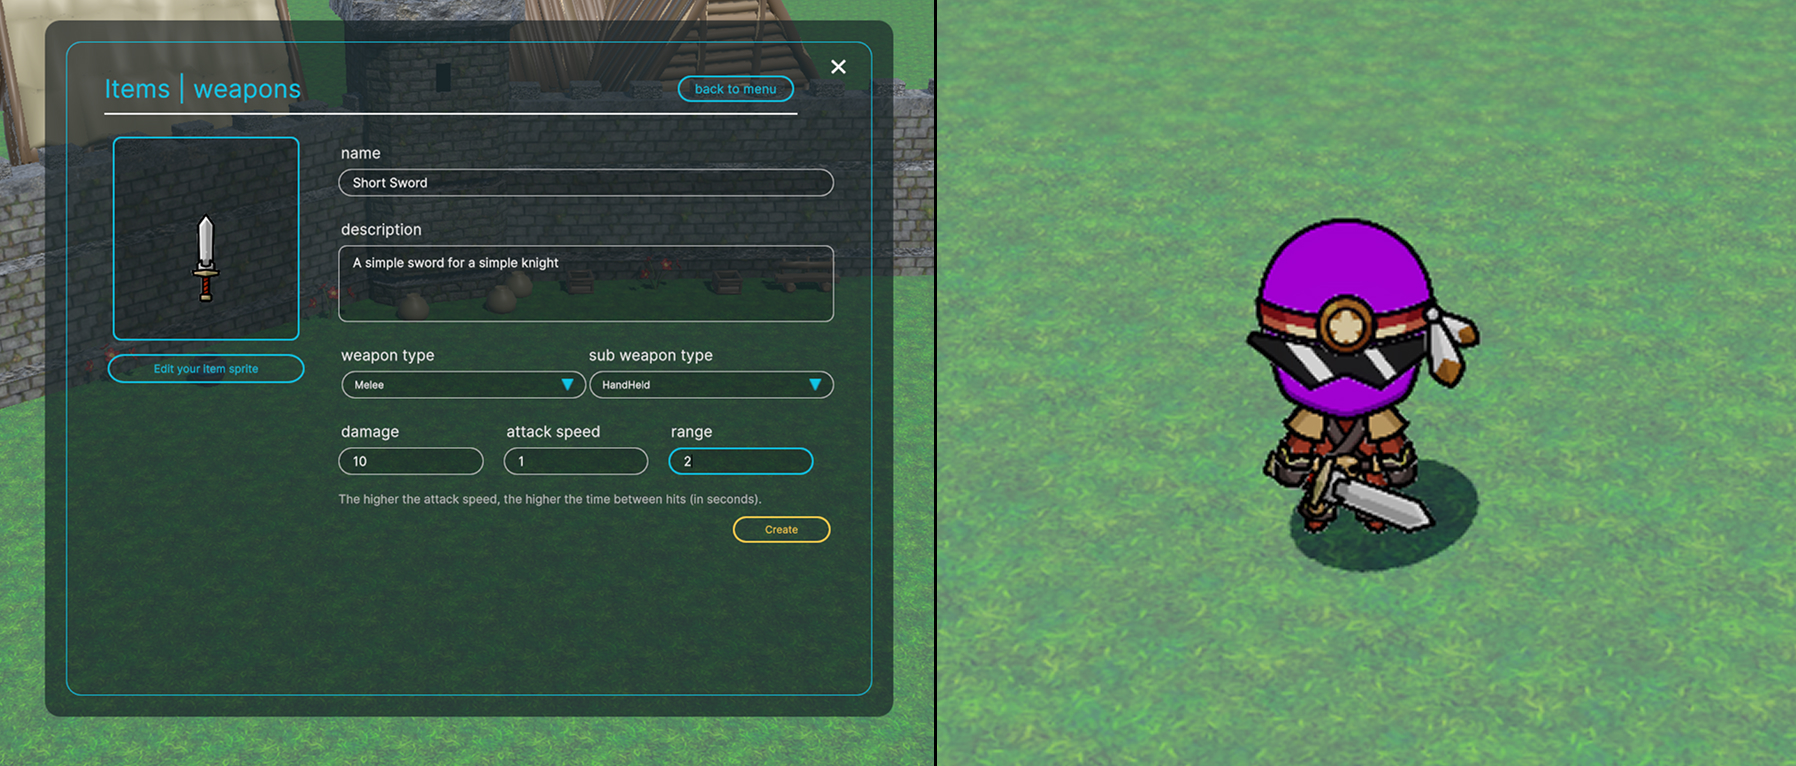
\includegraphics[width=0.9\textwidth]{img/08-implemented-solution/product/weapon-melee.jpg}
\caption{Captura de un jugador con una arma melee equipada y como se ve en el creador de mundos}
\end{figure}

\begin{figure}[H]
\centering
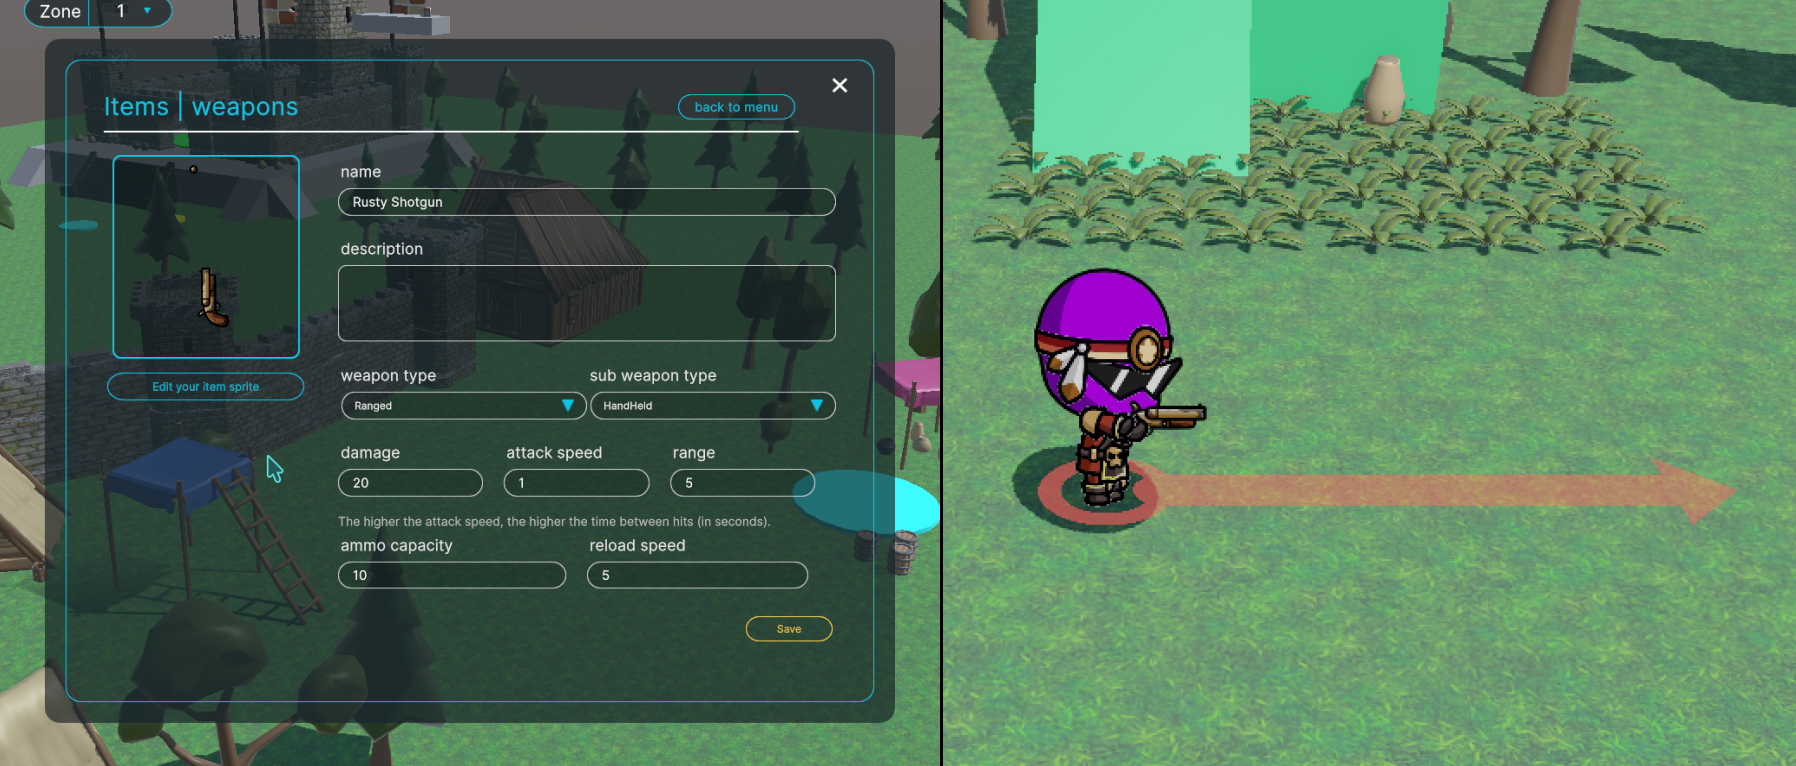
\includegraphics[width=0.9\textwidth]{img/08-implemented-solution/product/weapon-ranged.jpg}
\caption{Captura de un jugador con una arma a distancia equipada y como se ve en el creador de mundos}
\end{figure}

\subsubsection{Cosméticos}

Los cosméticos son elementos que los jugadores pueden equipar para personalizar la apariencia de su 
personaje sin afectar sus estadísticas ni habilidades. Los creadores pueden importar sus propios cosméticos para 
ofrecerlos a la venta a los jugadores. Eso se verá en mayor detalle en la sección de \textbf{Tiendas y Monetización}.

\begin{figure}[H]
\centering
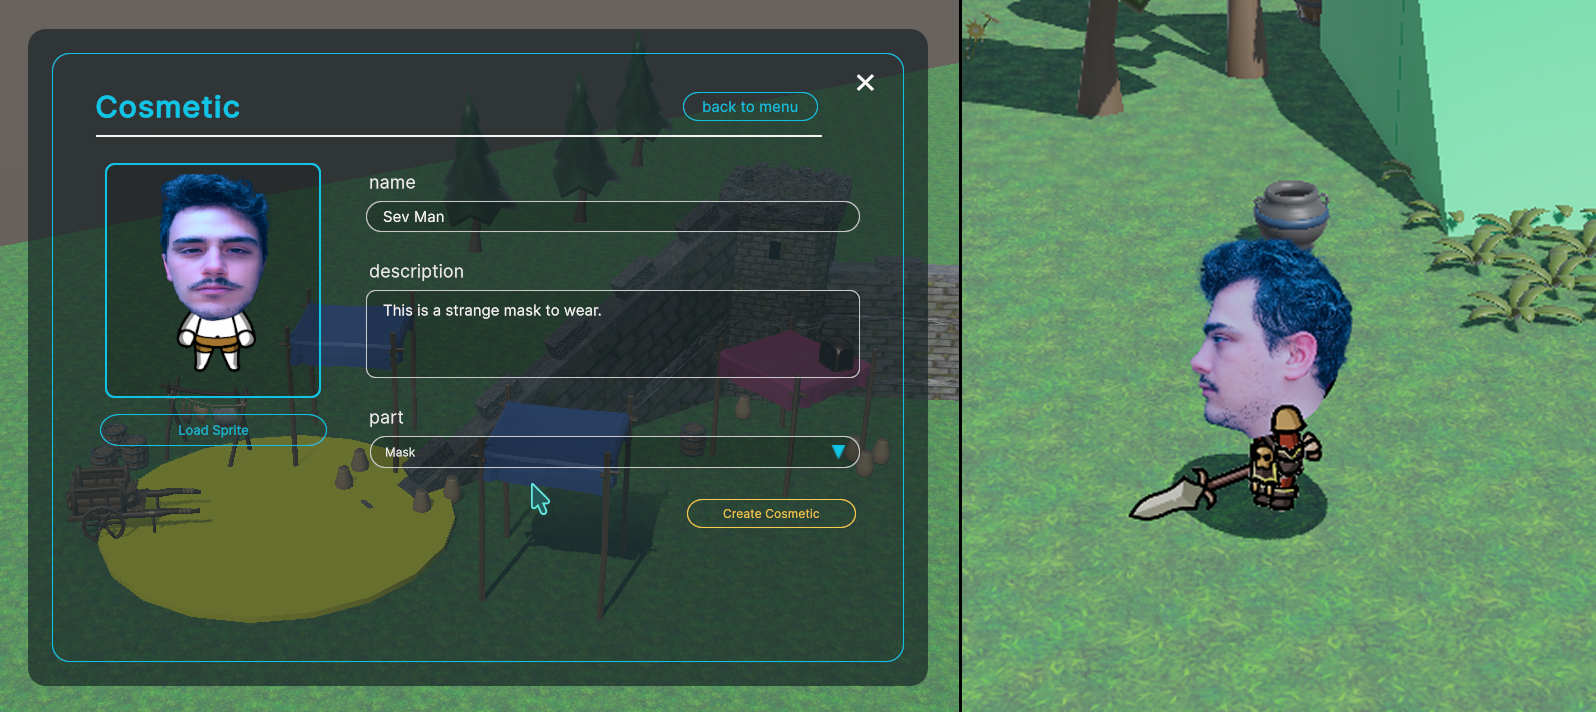
\includegraphics[width=0.9\textwidth]{img/08-implemented-solution/product/cosmetics.jpg}
\caption{Captura de un jugador con un cosmético equipado y como se ve en el creador de mundos}
\end{figure}

La única dificultad que puede surgir al importar cosméticos es que se requiere seguir un formato específico para 
que se rendericen correctamente en el juego. Por el momento no se ofrecen indicaciones sobre dichos formatos, ya 
que quedó fuera del alcance del MVP, pero se espera poder brindar a futuro una guía detallada para los creadores 
que deseen importar sus propios cosméticos.

\subsubsection{Tablas de recompensas}

Las tablas de recompensas (\textit{Loot Tables}) son configuraciones que determinan qué ítems pueden 
obtener los jugadores al interactuar con ciertos objetos del juego, como abrir cofres, matar enemigos ó al final de una expedición. Estas 
tablas permiten a los creadores definir la probabilidad de que un ítem específico sea otorgado como recompensa, 
así como el rango de oro que puede obtenerse.

\begin{figure}[H]
\centering
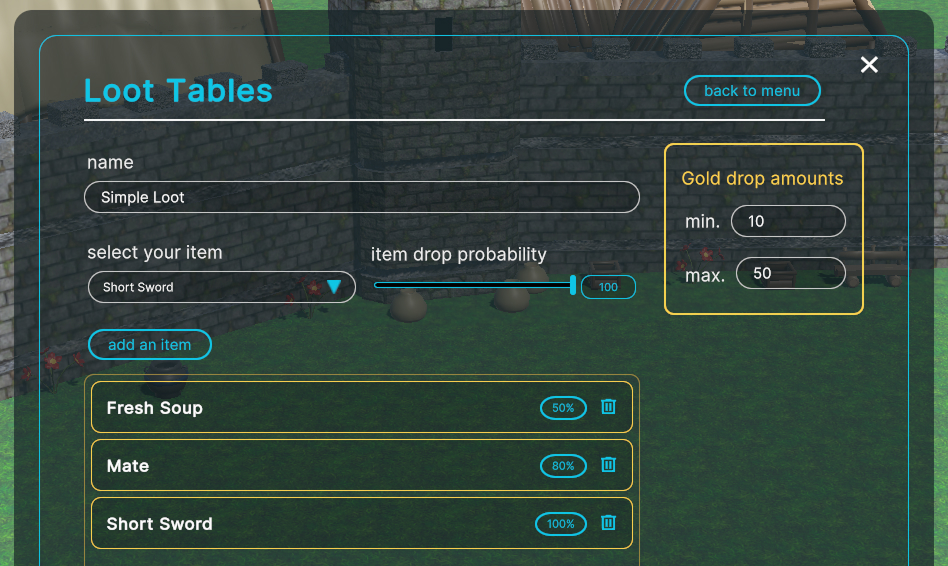
\includegraphics[width=0.8\textwidth]{img/08-implemented-solution/product/loot-table.jpg}
\caption{Captura de la configuración de una tabla de recompensas en el creador de mundos}
\end{figure}
